\documentclass[a4paper,10pt]{article}

\usepackage{tikz}
\usepackage{dblfnote}
\usepackage{lipsum}

\usepackage{geometry}
\geometry{
    right=1cm,
    left=1cm,
    top=2cm,
    bottom=2cm
}

\usepackage{xepersian}
\settextfont{Vazirmatn-Regular.ttf}

\title{سوالات احتمالی میان‌ترم 2 درس الگوریتم‌های گراف (با پاسخ)}
\author{استاد مربوطه:\\سرکار خانم دکتر معصومه دامرودی \and به نوشته:\\محمد خورشیدی روزبهانی}
\date{}

\linespread{1.5}

\begin{document}

    \maketitle

    \paragraph{سوال:} تعاریف، قضایا، نتایج و کاربردهای درون اسلایدها را شرح دهید.

    \paragraph{پاسخ:} اﺑﺘﺪا ﺑﻪ ﺗﻌﺎرﯾﻒ ﻣﻮﺟﻮد در اﺳﻼﯾﺪﻫﺎ پرداخته ﺷﺪه و ﻣﻮارد ﺑﻪ تفکیک ﺗﻮﺿﯿﺢ داده میﺷﻮد.

    \begin{itemize}
        
        \item ارتباطی/پیوندی\footnote{\hspace{2pt}Connectivity}: در مفهوم گراف، ارتباطی/پیوندی یک مفهوم مهم است که به ارتباط و ارتباطات بین رئوس در یک گراف اشاره دارد.

        \item اجزای متصل\footnote{\hspace{2pt}Components Connected}: در مفهوم گراف، اجزای متصل به زیرمجموعه‌هایی از رئوس در یک گراف اشاره دارند که هر راس در هر اجزای متصل قابل دسترسی به همه‌ رئوس دیگر آن اجزا است، اما با رئوس اجزا دیگر قابل دسترسی نیستند. به عبارت دیگر، هر اجزای متصل به گونه‌ای با هم ارتباط دارند که می‌توان از هر راس در یک اجزای متصل به هر راس دیگر در همان اجزای متصل مسیری یافت.
        
        این مفهوم در تجزیه و تحلیل گراف‌ها و برخی مسائل کاربرد دارد، زیرا اجزای متصل می‌توانند به عنوان واحدهای اصلی در بررسی ساختار یک گراف مورد استفاده قرار گیرند.
        
        \item اتصال\footnote{\hspace{2pt}Connectedness}: مفهوم اتصال در یک گراف به وجود داشتن مسیر بین هر زوج رئوس در گراف اشاره دارد. به عبارت دیگر، یک گراف متصل است اگر بین هر دو راس دلخواهی در آن یک مسیر وجود داشته باشد.

        اگر یک گراف یک اجزای متصل داشته باشد، به عنوان یک واحد اتصالی در نظر گرفته می‌شود و به عنوان یک واحد کلی مورد بررسی قرار می‌گیرد. اگر یک گراف دو یا چند اجزای متصل داشته باشد، این گراف به عنوان یک گراف قطع شده محسوب می‌شود.

        اتصال در گراف‌ها به ما اطمینان می‌دهد که ارتباطات بین رئوس یا نقاط در گراف حفظ شده است و هیچ رئوسی از دسترسی به همسایگان خود محروم نیست. این مفهوم در بسیاری از برنامه‌ها و مسائلی مانند شبکه‌ها، مسائل جستجو، طراحی سیستم‌های ارتباطی، و غیره کاربرد دارد.

        \item بسیار متصل\footnote{\hspace{2pt}Connected Strongly}: یک گراف جهت‌دار\footnote{\hspace{2pt}Graph Directed} را می‌توان به عنوان «بسیار متصل» توصیف کرد اگر برای هر زوج رئوس مختلف $u$ و $v$ در گراف، یک مسیر از $u$ به $v$ و یک مسیر از $v$ به $u$ وجود داشته باشد. به طور دیگر، اگر بتوانیم از هر راس به هر راس دیگری در گراف دسترسی پیدا کنیم، آن گراف را بسیار متصل می‌نامیم.

        مفهوم بسیار متصل در گراف‌های جهت‌دار بسیار مهم است، به ویژه در مسائلی که ارتباطات جهت‌دار بین نقاط مهم هستند، مانند مسائل راه‌یابی و تحلیل شبکه‌های ارتباطی.

        \item اجزای بسیار متصل\footnote{\hspace{2pt}Component Connected Strongly (SCC)}: در واقع، این اصطلاح به یک زیرگراف جهت‌دار\footnote{\hspace{2pt}Subgraph Directed} از یک گراف اشاره دارد که تمام رئوس آن به یکدیگر متصل هستند و از هر راسی به هر راس دیگری در آن زیرگراف مسیر وجود دارد.

        \item کلاس اولیه\footnote{\hspace{2pt}Class Initial}: این مفهوم به راس یا رئوسی درون هر اجزای متصل اشاره دارد که هیچ یال ورودی ندارند. به عبارت دیگر، رئوسی که دریافت یال از رئوس دیگر را نمی‌کنند. این رئوس به عنوان نقاط شروع دیده می‌شوند که از آنجا پیمایش‌ها و ارتباطات درون کامپوننت شروع می‌شود.

        \item کلاس پایانی\footnote{\hspace{2pt}Class Final}: این مفهوم به راس یا رئوس درون هر اجزای متصل اشاره دارد که هیچ یال خروجی ندارند. به عبارت دیگر، رئوسی که هیچ یالی به رئوس دیگر بیرون از کامپوننت ارسال نمی‌کنند. این رئوس به عنوان نقاط پایانی مورد استفاده قرار می‌گیرند که پایان یافتن پیمایش‌ها و ارتباطات را نشان می‌دهند.
        
        \item کلاس میانی\footnote{\hspace{2pt}Class Intermediate}: راس یا رئوسی که هم یال ورودی و هم یال خروجی دارند و درون هر اجزای متصل وجود دارند، به عنوان رئوس میانی شناخته می‌شوند. این رئوس به عنوان مسیرهای انتقالی بین نقاط شروع و پایان درون یک کامپوننت عمل می‌کنند.

        \item برش راسی\footnote{\hspace{2pt}Vertex-Cut}: مفهوم برش راسی در گراف، یک مجموعه‌ای از رئوس یا گره‌ها است که با حذف آن‌ها، گراف به دو یا چندین قسمت جداگانه تقسیم می‌شود. به طور دقیق‌تر، اگر حذف یک مجموعه از رئوس باعث شود که گراف دیگر به‌طور متصل نباشد، آن مجموعه به عنوان یک برش رأسی شناخته می‌شود.
        
        \begin{center}
            
            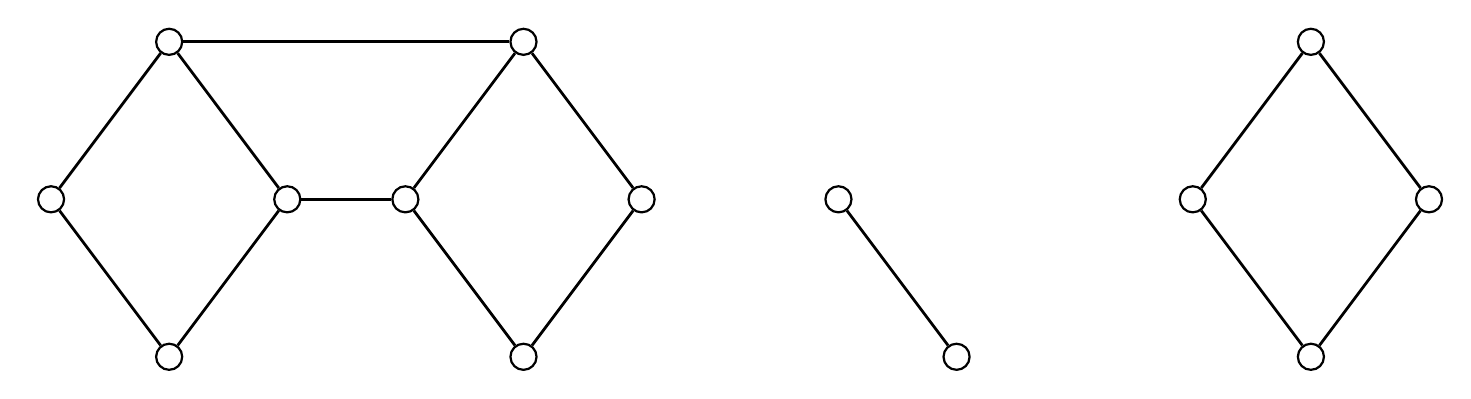
\begin{tikzpicture}

                \node[circle, draw, thick] (A) at (0,0) {};
                \node[circle, draw, thick] (B) at (1.5,2) {};
                \node[circle, draw, thick] (C) at (1.5,-2) {};
                \node[circle, draw, thick] (D) at (3,0) {};
                \node[circle, draw, thick] (E) at (4.5,0) {};
                \node[circle, draw, thick] (F) at (6,2) {};
                \node[circle, draw, thick] (G) at (6,-2) {};
                \node[circle, draw, thick] (H) at (7.5,0) {};
                
                \draw[line width=1pt] (A) -- (B);
                \draw[line width=1pt] (A) -- (C);
                \draw[line width=1pt] (B) -- (D);
                \draw[line width=1pt] (C) -- (D);
                \draw[line width=1pt] (E) -- (F);
                \draw[line width=1pt] (E) -- (G);
                \draw[line width=1pt] (F) -- (H);
                \draw[line width=1pt] (G) -- (H);
                \draw[line width=1pt] (B) -- (F);
                \draw[line width=1pt] (D) -- (E);

                \node[circle, draw, thick] (A) at (10,0) {};
                \node[circle, draw, thick] (C) at (11.5,-2) {};
                \node[circle, draw, thick] (E) at (14.5,0) {};
                \node[circle, draw, thick] (F) at (16,2) {};
                \node[circle, draw, thick] (G) at (16,-2) {};
                \node[circle, draw, thick] (H) at (17.5,0) {};

                \draw[line width=1pt] (A) -- (C);
                \draw[line width=1pt] (E) -- (F);
                \draw[line width=1pt] (E) -- (G);
                \draw[line width=1pt] (F) -- (H);
                \draw[line width=1pt] (G) -- (H);

            \end{tikzpicture}

        \end{center}

        \item برش یالی\footnote{\hspace{2pt}Edge-Cut}: در مفهوم گراف، یک برش یالی مجموعه‌ای از یال‌ها است که با حذف آن‌ها، گراف به دو یا چندین قسمت جداگانه تقسیم می‌شود. به طور دقیق‌تر، اگر حذف یک مجموعه از یال‌ها باعث شود که هیچ مسیری بین دو راس در دو قسمت متفاوت از گراف وجود نداشته باشد، آن مجموعه به عنوان یک برش یالی شناخته می‌شود.

        \begin{center}
            
            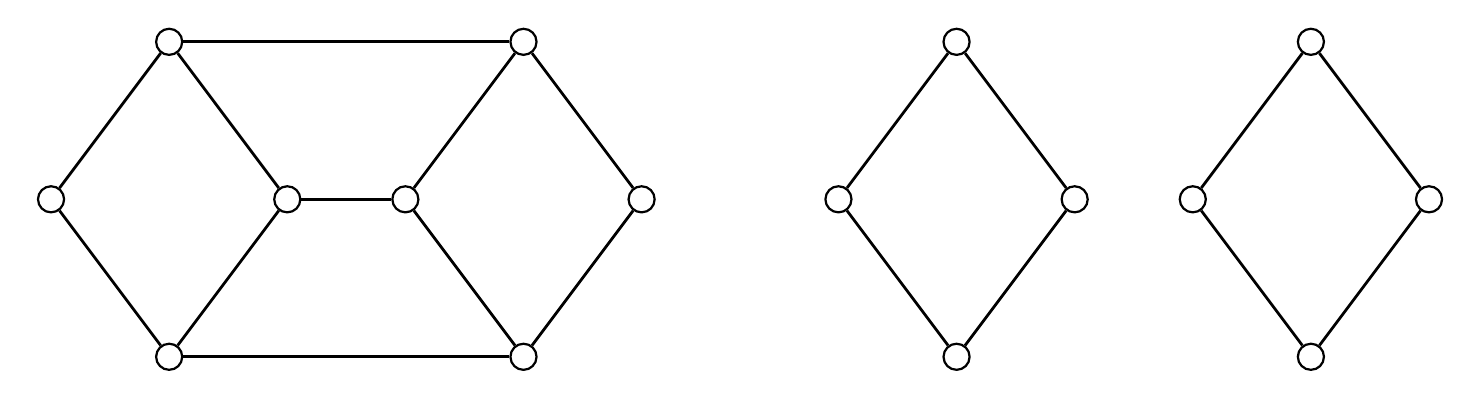
\begin{tikzpicture}

                \node[circle, draw, thick] (A) at (0,0) {};
                \node[circle, draw, thick] (B) at (1.5,2) {};
                \node[circle, draw, thick] (C) at (1.5,-2) {};
                \node[circle, draw, thick] (D) at (3,0) {};
                \node[circle, draw, thick] (E) at (4.5,0) {};
                \node[circle, draw, thick] (F) at (6,2) {};
                \node[circle, draw, thick] (G) at (6,-2) {};
                \node[circle, draw, thick] (H) at (7.5,0) {};
                
                \draw[line width=1pt] (A) -- (B);
                \draw[line width=1pt] (A) -- (C);
                \draw[line width=1pt] (B) -- (D);
                \draw[line width=1pt] (C) -- (D);
                \draw[line width=1pt] (E) -- (F);
                \draw[line width=1pt] (E) -- (G);
                \draw[line width=1pt] (F) -- (H);
                \draw[line width=1pt] (G) -- (H);
                \draw[line width=1pt] (B) -- (F);
                \draw[line width=1pt] (D) -- (E);
                \draw[line width=1pt] (C) -- (G);

                \node[circle, draw, thick] (A) at (10,0) {};
                \node[circle, draw, thick] (B) at (11.5,2) {};
                \node[circle, draw, thick] (C) at (11.5,-2) {};
                \node[circle, draw, thick] (D) at (13,0) {};
                \node[circle, draw, thick] (E) at (14.5,0) {};
                \node[circle, draw, thick] (F) at (16,2) {};
                \node[circle, draw, thick] (G) at (16,-2) {};
                \node[circle, draw, thick] (H) at (17.5,0) {};
                
                \draw[line width=1pt] (A) -- (B);
                \draw[line width=1pt] (A) -- (C);
                \draw[line width=1pt] (B) -- (D);
                \draw[line width=1pt] (C) -- (D);
                \draw[line width=1pt] (E) -- (F);
                \draw[line width=1pt] (E) -- (G);
                \draw[line width=1pt] (F) -- (H);
                \draw[line width=1pt] (G) -- (H);

            \end{tikzpicture}

        \end{center}

        \item 

    \end{itemize}

\end{document}